\documentclass[a4paper, 12pt, oneside]{scrbook}
\usepackage[hyphens,spaces,obeyspaces]{url}
\usepackage[sorting = none, backend=bibtex]{biblatex}
\usepackage[german]{babel}
\usepackage[T1]{fontenc}
\usepackage[utf8]{inputenc}
\usepackage[hidelinks]{hyperref}
\usepackage{graphicx}
\usepackage{subcaption}
\usepackage{epstopdf}
\usepackage{lmodern}
\usepackage{float}
\usepackage{acronym}
\usepackage{booktabs}
\usepackage{caption}
\usepackage{csquotes}
\usepackage{enumitem}
\usepackage{fancyhdr}
\usepackage{url}
\usepackage{listings}
\usepackage[table]{xcolor}
\usepackage{wrapfig}
\usepackage{forest}
\usepackage{tabularx}
\usepackage{colortbl}
\usepackage{booktabs}
\usepackage[onehalfspacing]{setspace}
\usepackage{amsmath}
\usepackage{threeparttable}
\usepackage[german]{cleveref}
\usepackage{parskip}

\renewcommand*{\headfont}{\normalfont}
\renewcommand*{\multicitedelim}{\addsemicolon\space}
\renewcommand*{\headrulewidth}{0pt}
\renewcommand*{\arraystretch}{1.5}
\setlength{\parskip}{1.5ex}
\makeatletter
% define new boolean conditional switch for whether
% the abstract is being typeset
\newif\ifabstract
% redefine `\chapter` so it only starts a new page if not typesetting
% the abstract; sets abstract conditional to false after doing so
\renewcommand\chapter{\ifabstract\relax\else%
	\if@openright\cleardoublepage\else\clearpage\fi%
	\fi
	\abstractfalse%
	\thispagestyle{plain}%
	\global\@topnum\z@
	\@afterindentfalse
	\secdef\@chapter\@schapter}

% command for putting the title and name above the abstract; switches
% abstact boolean to true for next `\chapter*` command...
\newcommand{\conclusion}{
	\if@openright\cleardoublepage\else\clearpage\fi
		\begin{center}
			\textbf{\larger{Summary}}\par
			\emph{Hier kommt nach der Fertigstellung der Arbeit noch eine Zusammenfassung der Arbeit mit ein oder mehreren Sätzen hin. Hier kommt nach der Fertigstellung der Arbeit noch eine Zusammenfassung der Arbeit mit ein oder mehreren Sätzen hin. Hier kommt nach der Fertigstellung der Arbeit noch eine Zusammenfassung der Arbeit mit ein oder mehreren Sätzen hin2. }\par
		\end{center}

	\abstracttrue}
\makeatother
\lstset
{
         basicstyle=\footnotesize\ttfamily,
         numbers=left,               	% Ort der Zeilennummern
         numberstyle=\tiny,          	% Stil der Zeilennummern
%         stepnumber=2,               	% Abstand zwischen den Zeilennummern
         numbersep=5pt,              	% Abstand der Nummern zum Text
         tabsize=2,                  	% Groesse von Tabs
         extendedchars=true,
         breaklines=true,            	% Zeilen werden Umgebrochen
         keywordstyle=\color{red},
            frame=b,
 %        keywordstyle=[1]\textbf,    	% Stil der Keywords
 %        keywordstyle=[2]\textbf,
 %        keywordstyle=[3]\textbf,
 %        keywordstyle=[4]\textbf, \sqrt{\sqrt{}}
         stringstyle=\color{white}\ttfamily,
         showspaces=false,
         showtabs=false,
         xleftmargin=27pt,
         framexleftmargin=27pt,
         framexrightmargin=5pt,
         framexbottommargin=4pt,
%         backgroundcolor=\color{lightgray},
         showstringspaces=false      	% Leerzeichen in Strings anzeigen ?
}
\addbibresource{Bachelorarbeit.bib}

\begin{document}
	\frontmatter
	\def\doctype{Bachelorarbeit}
\def\title{Vorgehensweise zur Implementierung der VDMA Spezifikation „OPC UA for Machinery (OPC 40 001)“ in Maschinen und IT-Systemen erarbeiten}
\def\author{Rico Kursidem}
\def\supervisor{Dipl. Ing (FH) Michalowski}
\def\supervisortwo{Prof. Dr. Mielebacher}

\begin{titlepage}

\vspace{10mm}

\begin{center}
	
	\vspace{5mm}
	\huge \title
	
	\vspace{34pt}
	\large \doctype
		
	\vspace{30pt}	
	\small Angewandte Informatik \\
	\large Duale Hochschule Baden-Württemberg Mosbach \\
	\small Studienpartner \\
	\large AZO GmbH \& Co. KG \\
    \vspace{35pt}
    
    
\includegraphics[height=2.5cm]{prefix/image/logo-dhbw.eps}
    
\includegraphics[height=2.5cm]{prefix/image/logo-azo.png}
	
	\vspace{40pt}	
	\small von \\
	\large \author \\
	\small betreut von \\
	\large \supervisor \\
	\small und \\
	\large \supervisortwo

\end{center}

\vspace{75pt}


\vspace{49.7pt}

\fancypagestyle{empty}{
  \fancyhf{}
  \fancyfoot[C]{\today}
}

\end{titlepage}
	\chapter*{Abkürzungsverzeichnis} 
\begin{acronym}
	%A
	\acro{API}{Advanced Programming Interface}
	%B
	%C
	\acro{COM}{Component Object Model}
	%D
	\acro{DCOM}{Distrebuted Component Object Model}
	%E
	\acro{ERP}{Enterprse Recource Planning}
	%F
	%G
	%H
	\acro{HMI}{Human Maschine Interface}
	%I
	\acro{IoT}{Internet of Things}
	%J
	%K
	%L
	%M
	\acro{M2M}{Maschine-zu-Maschine}
	\acro{MES}{Manufacturing Execution System}
	\acro{MQTT}{Message Queuing Telemetry Transport}
	%N
	%O
	\acro{OPC UA}{Open Platform Communications Unified Architecture}
	%P
	%Q
	%R
	%S
	\acro{SOA}{Service orientierte Architektur}
	%T
	\acro{TCP/IP}{Transmission Control Protocol/Internet Protocol}
	%U
	\acro{UMATI}{Universal machien technology interface}
	%V
	\acro{VDMA}{Verband Deutscher Maschinen- und Anlagenbau}
	\acro{VDW}{Verein Deutscher Werkzeugmaschinenfabriken e.V. }
	%W
	%X
	%Y
	%Z
\end{acronym}
	\tableofcontents
	\listoffigures
	\listoftables
	%\lstlistoflistings
	\nocite{*}

	\mainmatter
	
	\chapter*{Abstract}
	
	\section*{Deutsch}
	
	
	\section*{English}
	
	\pagebreak
%	\conclusionpng
	\chapter{Einführung}
	% (4 Seiten)
	
	% Hinführung
	% M2M - Kommunikation
	% vertikale Integration
	% Industrie 4.0
	% added Value to data
	% automated posibilities
	
	% Lesermotivation 
	
	\section{Problemstellung und Ziel}
	
	% (1-2 Seiten)
	
	 Durch die zunehmende Automatisierung der Produktion und Fertigung stehen viele Produzenten vor der Aufgabe, zahlreiche Maschinen verschiedenster Hersteller in ihren Fertigungsprozess zu integrieren. Viele dieser Maschinen nutzen verschiedene Kommunikationsprotokolle, Datenformate und Schnittstellen was die Integration dieser diversen Systeme erschwert. Durch eine komplizierte Integration kann Vendor Locking entstehen. Die Bindung eines Kunden an einen Anbieter, da dieser eine Technologie Integriert, die andere Hersteller nicht oder nur extrem Schwer Integrieren können. Dies kann zu einer Atmosphäre führen, welche für den Kosten weniger Flexibilität und Kontrolle über seine eigene Produktion gibt und gleichzeitig die Kosten steigen lässt. Um dieses Problem zu lösen müssen sich die Produzenten zu einem Standard zusammenfinden und die Interoperabilität ihrer Systeme gewährleisten.
	
	 Für AZO als Anlagenproduzent ist es von großem Interesse mit Anlagen und Maschinen anderer Hersteller kommunizieren zu können und dabei die Integration möglich einfach zu realisieren. Auch für Entwickler von \ac(MES) bedeutet die Standardisierung von Kommunikationsprotokollen eine schnellere und einfachere Entwicklung was zu niedrigeren Entwicklungskosten führt und die Robustheit der Systeme erhöhen kann. AZO hat, um diese Standardisierung zu erreichen, an der Ausarbeitung von \ac{UMATI} zugesagt. Dieser Standard möchte die Kommunikation zwischen Maschinen und der darüber liegenden Datenverarbeitung definieren und basiert auf dem Offenen Standard \ac{OPC UA}.
	
	 Das Ziel dieser Arbeit ist es, UMATI in einem Testumfeld aufzubauen und eine Proof of Konzept System aufzubauen. Um dies zu erreichen soll zunächst eine Marktanalyse durchgeführt werden und mögliche Lösungen zum versenden und empfangen von Daten zwischen Maschine und MES zu finden. Diese sollen anhand von selbst entwickelten Kriterien abgewogen und bewertet werden. Die vielversprechendsten Umsetzungen sollen in einem Testsystem implementiert werden und für zukünftige Demonstrationen auf Messen für AZO zur Verfügung gestellt werden. Außerdem soll evaluiert werden, ob UMATI auch in der Low-Code Plattform Node Red angewendet werden kann und wenn möglich, das entstehende System als Open-Source Lösung der Öffentlichkeit zur Verfügung zu stellen.
	
	 Der Prototyp soll ebenfalls eine Integration in ACAS umfassen. Damit kann gezeigt werden, dass UMATI eine Möglichkeit ist, die Kommunikation von AZO Anlagen und ACAS zu realisieren. Diese Integration muss im Nachgang weiter Evaluiert werden um festzustellen ob UMATI als Standardisierung eine gute Lösung ist.
	
	%TODO Relevanz für AZO und Wissenschaft
	%TODO Sicherheitsrelevanz
	
	\section{Unternehmen}
	
	 Diese Arbeit wird mit dem Dualen Partner \textit{AZO Gmbh \& Co. KG} durchgeführt. AZO bietet maßgeschneiderte Lösungen für die automatisierte Förderung, Lagerung und Dosierung von Rohstoffen weltweit an. Dabei werden Anlagen für die Bereiche der Chemie-, Nahrungsmittel-, Pharma-, Kosmetik und Kunststoffindustrie gefertigt. Diese Projekte umfassen die Planung, Fertigung und Montage, sowie die Automatisierung der Anlagen.
	
	 AZO entwickelt ein eigenes MES System ACAS, welches die Kommunikation zwischen Anlagen von AZO, aber auch Anlagen von anderen Herstellern, mit den Kunden vereinheitlichen und verbessern soll. Dabei soll ein Umfassendes System entstehen, welches Steuerung, Visualisierung und Überwachung der Produktion übernehmen und in einer zentralen Software bündeln soll.
	
	 ACAS entsteht in der Entwicklungsabteilung welche ebenfalls an dieser Arbeit beteiligt ist. Sie fokussiert sich auf die Automatisierung von AZO Anlagen im Bereich von SPS Steuerungen bis zur Datenverarbeitung und Erhebung auf abstrahierter Ebene. 
	
	%TODO: Was stellt mir AZO zur verfügung - System, Server, ...
	
	\section{Forschungsfragen}
	
	Die Standardisierung der Integration von verschiedensten Maschinen in eine Umgebung ist nötig und kann zu verstärkten Effizienzsteigerungen und Aufwandsersparnis führen. Für Anlagenbauer verspricht die Nutzung von Umati, diese Integration in einen schnellen und effizienten Prozess zu wandeln. Um das Potential von Umati zu evaluieren wurden folgende Schwerpunkte betrachtet:
	
	\begin{itemize}
		\item \textbf{Q1}: Welche Herausforderungen ergeben sich bei der Umsetzung von Umati?
		\item \textbf{Q2}: Welche Lösungen zur Umsetzung von Umati sind am Wirtschaftlichsten?
		\item \textbf{Q3}: Wie kann die Datenkommunikation von Anlage und ACAS bestmöglich implementiert werden?
	\end{itemize}
	
	\section{Aufbau der Arbeit}
	
	% Methodik - kurz
	% Aufbau ->
		% Analyse: Marktanalyse und Informationssammlung über Lösungen
		% Implementierung des Prototypen
		% Integration in ACAS
		% Erstellen von Materialien für Messen und Demos
				% Schulung des Personals
	
\chapter{Grundlagen}
	% (16 Seiten)
	
	% Stand der Technik
	
	
	\section{OPC UA}
	
	%OPC UA
	% - Interoperabilität
	
	% Aufbau
	% Aufgaben
	% Standards und Anforderungen
	
	 \ac{OPC UA} ist ein Unternehmensunabhängiger, offener Standard zur Kommunikation von Informationen und Daten zwischen Maschinen im Industriellen Umfeld. Das Protokoll wurde 2008 von der OPC Foundation veröffentlicht und nimmt sich zur Aufgabe, die Interoperabilität von Systemen zu fördern. Es verwendet eine Service orientierte Architektur und kann auf verschiedensten Betriebssystemen verwendet werden. OPC UA ist sehr gut Skalierbar und kann deshalb als Kommunikationsprotokoll bei kleinen \ac{IoT} Systemen als auch bei komplexen Cloud Systemen zur Anwendung kommen.
	
	 OPC UA baut auf einem Server-Client-Modell auf, wobei der Client die Anfragen an den Server senden muss. Der Client fragt den Server nach Daten und analysiert diese währen der Server stellt die Daten zur Verfügung. Diese Struktur ermöglicht eine einfache Skalierung von verschiedensten Geräten. 
	
	% TODO Hier muss noch was zwischen
	
	
	 Das Ziel von OPC UA und auch im weitergetragenen Sinne von Umati ist das erreichen von Interoperabilität im Industriellen Bereich. Interoperabilität beschreibt die Standardisierung von Kommunikation zwischen Systemen. Allgemein kann diese in 4 Stufen eingeteilt werden wobei jede Ebene auf die darunterliegende aufbaut. Im Schaubild \ref{fig:Interoperabilität} sind die vier Ebenen Strukturelle, Syntaktische, Semantische und Organisatorische Interoperabilität abgebildet.
	
	\begin{figure}[h]
		\centering
		\includegraphics[width=0.9\textwidth]{res/diagramms/Interoperabilität.pdf}
		\caption{Die vier Ebenden der Interoperabilität}
		\label{fig:Interoperabilität}
	\end{figure}

	Die strukturelle Interoperabilität beschreibt Verbindungen zwischen den Systemen weshalb sie auch oft als Konnektivität bezeichnet wird. Der Datenaustausch kann nur erfolgen wenn die beteiligten System miteinander Verbunden sind und ein geeignetes \ac{API} implementieren. Diese Verbundenheit kann über ein Netzwerk mit TCP/IP oder HTTP erreicht werden oder kann ein Übertragungsmedium wir USB festlegen.
	
	Sind Systeme syntaktisch Interoperabel, nutzen und verstehen sie die Struktur der Daten. Hierfür können festgelegte Standards wie XML oder Json verwendet werden. 
	
	Die Semantische Interoperabilität beschreibt das vereinheitlichte Verständnis der Daten. Kommunizieren zwei Systeme miteinander, so müssen Sie unter den Selben Daten auch das selbe Verstehen. Ein Beispiel für einen Standard der Semantische Interoperabilität umsetzt ist der "International Classification of Diseases". Bei diesem geht es um die Kommunikation von Krankheiten zwischen Ärzten und wurde von der WHO eingeführt. Jede Krankheit hat einen festgelegten Code, wodurch eine eindeutige Kommunikation gewährleistet ist.
	
	OPC UA legt anhand des Information Models den Syntax und die Semantik der Daten fest, wodurch die syntaktische Interoperabilität gewährleistet ist. Die semantische Interoperailität wird anhand der Companion Standards erweitert. Diese beschreiben Technologie-spezifische Informationsmodelle. Diese Standards entstanden durch intensive Kooperation und Zusammenarbeit mit Organisationen um die Standards möglichst umfassend aufzustellen. %\cite{}
	
	OPC UA entstand aus dem zuvor entwickelten Standard OPC Classics. Der alte Standdard setzte die Kommunikation im Bereich der Automatisierung bereits sehr gut um. Der Nachteil an Classics war jedoch die fehlende Plattformunabhängigkeit. OPC UA unterstützt heute jegliche Betriebsysteme für Clients als auch für die Server. Der Vorgänger musste auf einem Windowssystem betreiben werden. Auch die Kommunikation war auf die von Microsoft entwickelte Technologien \ac{COM} und \ac{DCOM} basiert. Durch die Ablösung dieses Standards durch OPC UA wird über TCP/IP und SOAP kommuniziert, welche beide Plattformunabhängig sind und somit kann zunehmend OPC UA auch auf anderen Plattformen wie Linux, Mac und Android angewandt werden.
	
		\subsection{Companion Spezifikationen}
		
		
		
		\begin{figure}[h]
			\centering
			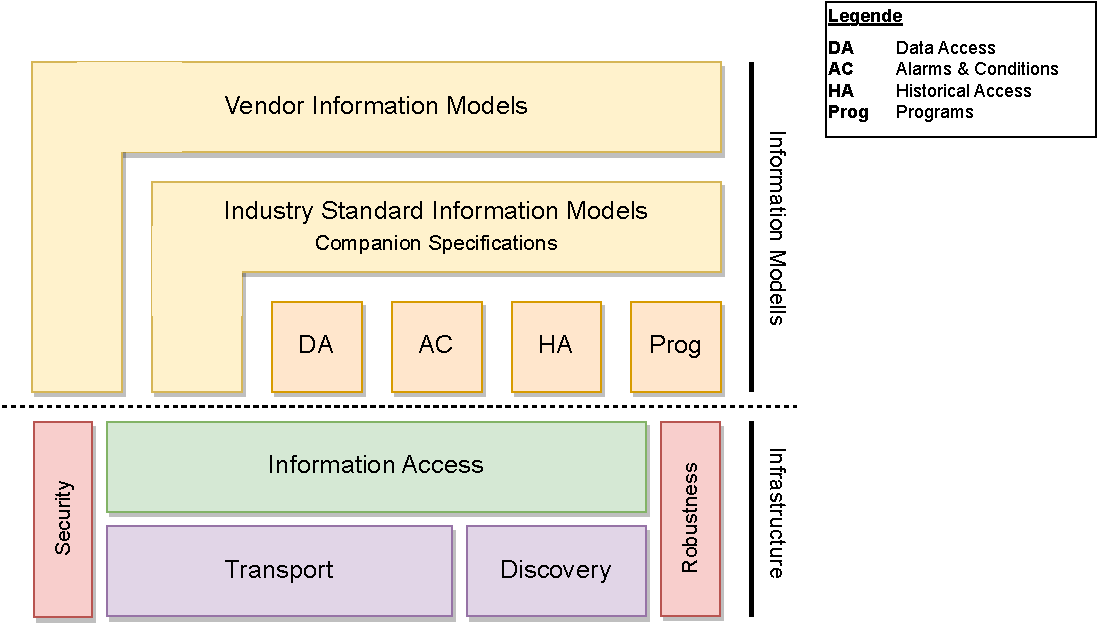
\includegraphics[width=0.9\textwidth]{res/diagramms/companionSpezifikations.pdf}
			\caption{Aufbau des OPC UA Standards, \\ Angelehnt an: http://wiki.opcfoundation.org/images/8/8c/UA\_Framework.JPG} %TODO anständig machen
			\label{fig:OPCUA_Framework}
		\end{figure}
	
		\subsection{Architektur} % Noch nicht Final: Struktur? Aufbau?
		
		OPC UA besteht aus drei Komponenten deren Zusammenwirkung in Abbildung \ref{fig:OPCUA_Structure} abgebildet ist. Mehrere Field Connections, die die Sensorik oder SPS darstellen mit welchen kommuniziert werden soll. Die Daten sollen zu den OPC UA Clients geleitet werden. Dies können \ac{HMI} oder MES Systeme sein, die die Daten der Maschinen auswerten oder Steuerungsbefehle absenden möchten. OPC UA Standardisiert diese Kommunikation über den OPC UA Server. Dieser setzt den OPC UA Standard um und stellt die notwendigen APIs zur Verfügung.
		
		\begin{figure}[h]
			\centering
			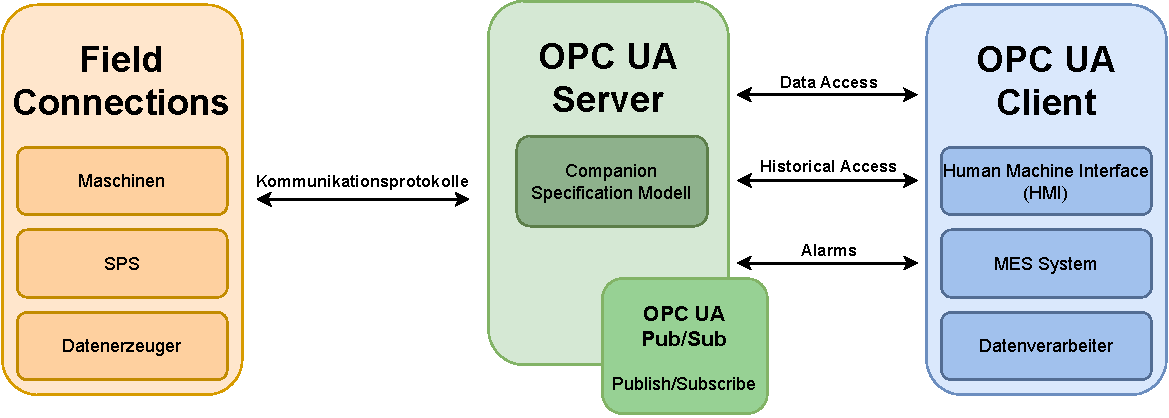
\includegraphics[width=0.9\textwidth]{res/diagramms/OPCUA.pdf}
			\caption{Kommunikationsstruktur OPC UA}
			\label{fig:OPCUA_Structure}
		\end{figure}
		
		Der OPC UA Server implementiert die proprietären Kommunikationsprotokolle, die vom Maschinenhersteller entwickelt wurden, um mit den Anlagen und den Field Conections zu Kommunizieren. Je nach art der Daten die die Maschine weiter gibt, werden die Daten auf dem OPC UA Server abgespeichert oder an den Client weiter gegeben. Ein OPC UA Server kann in zwei Formen entstehen. Der Hersteller kann seiner Maschine die OPC UA Standards bereits bei der Entwicklung einprogrammieren. Damit ist der Server in der Maschine integriert und die Maschine ist so von beginn an OPC UA fähig. Sollte der Hersteller die Spezifikationen jedoch nicht implementieren, kann der Server auch zusätzlich zwischen die Maschine und den Client geschallten werden. Durch die Unabhängigkeit des Herstellers sind diese Server oft mit mehr Kommunikationsprotokollen ausgestattet, was deren Möglichkeiten mit der Maschine zu interagieren erhöht. 
		
		Die Kommunikation mit dem Client läuft dabei 1 zu 1 ab. Allerdings kann auch ein 1 zu n Kommunikationsmodell über Publish and Subscribe implementiert werden. Um diese Funktion jedoch zu nutzen, muss der Server mit der OPC UA Pub/Sub Spezifikation erweitert werden.
		
		Der Client kann die Daten über die standardisierte API des OPC UA Servers abfragen. Es können Echtzeitdaten, Historische Daten abgerufen werden. Außerdem gibt es eine Spezifikation, wie Alarmierungslogik umgesetzt werden soll. Dies wird anhand der Implementation auf Serverebene deutlich vereinfacht, da sie dann Hersteller unabhängig ist.
		
		
		
		\subsection{Sicherheit}
		
		%TODO Security beschreiben
		% Wenn bei Umati sich etwas ändert, dann dort noch ein Kapitel puschen
	
	\section{Umati}
	
		% - Automatisierungspyramide
	
		\subsection{VDMA}
		\subsection{Anforderungen}
		\subsection{OPC UA 40001}
		
		% Was ist UMATI (Ziel, Entstehung, Stand der Technik)
		% OPCUA 40001
			% Was wird benötigt zum ...
				% senden
				% empfangen
			% Anmeldung
		
		% Marktanalyse: Bereits vorhandene Lösungen	
	
\chapter{Methodik}
	% (8 Seiten)
	
	
	% Forschungsmethodik - Deduktiv??? - Konstruktiv???
	
	\section{Literaturrecherche}
	% Datenerhebung - Literaturrecherche
	% Stichwort recherche
	
	\section{Evaluation}
	
	\section{Experteninterview}
	
	\section{Zeitplanung}
	
\chapter{Ergebnisse}
	
	% (8 Seiten)
	
	\section{Anforderungsanalyse}
	
	\section{Lösungsansätze}
		% Nach was suche ich, Kriterienentwurf
		% Was bracuh ich Hard Soft
		
		% Literaturrecherche an anderen Implementationen (Umati und 5G)
	
	\section{Marktanalyse}
	
		% Fertige Lösungen
		% Node Red selbstimplementierung
	
	\section{Wirtschaftlichkeit und Projektanalyse}
	
		\subsection{Kostenplanung}
		
		\subsection{Fallbeispiel}
			% Beispielswiese an Fallbeispiel -> Durchschnittliche AZO Straße
			% Interview mit Person die diese Integration macht -> Expertenquellen
			% -> Probleme bei Schnittstellen integrierung.
	
	\section{Implementierung eines Prototyps}
	
		\subsection{Aufbau der Umgebung}
		
		\subsection{Implementierung}
		
			% Proof of Konzept
			% Proof of Konzept mit Node Red
			
			% Probleme und Lösungen
		
		\subsection{Integration in bestehende Infrastruktur}
			% Integration in Unternehmensstruktur
			

	
	
	\chapter{Diskussion und Fazit}
	
		% (2-5 Seiten)	
	
		% Disskussion -> Subjektive Bewertung der Spezifikation UMATI, ... Literaturpunkte meine Meinung, Sinnvoll Einzusetzen
	
	
	\frontmatter
	\printbibliography

\end{document}
